\documentclass{article}
\usepackage{microtype}
\usepackage{graphicx}
\usepackage{subfigure}
\usepackage{booktabs} % for professional tables
\usepackage{hyperref}
\newcommand{\theHalgorithm}{\arabic{algorithm}}

\usepackage[accepted]{icml2019}

\icmltitlerunning{Neural Ordinary Differential Equations}

\begin{document}

\twocolumn[
\icmltitle{Neural Ordinary Differential Equations}
\icmlsetsymbol{equal}{*}

\begin{icmlauthorlist}
\icmlauthor{Weijie Gan}{equal,to}
\icmlauthor{Zayid Oyelami}{equal,to}
\end{icmlauthorlist}

\icmlaffiliation{to}{Washington Univ. in St.Louis}

\icmlcorrespondingauthor{Weijie}{weijie.gan@wustl.edu}
\icmlcorrespondingauthor{Zayid}{zzoyelam@gmail.com}

\icmlkeywords{Machine Learning, ICML}
\vskip 0.3in
]

\printAffiliationsAndNotice{\icmlEqualContribution} % otherwise use the standard text.

\begin{abstract}
    A new family of deep-learning, especially in recurrent neutral network (RNN), is introduced using differential equations. Instead of simply passing a layer to the next phase, the value of a layer is computed by solving a differential equations via a black-box-based algorithm. Effectively, the use of ODEs in neural networks is known as NODE. The utility of this method was tested in several experiments to exhibit constant memory cost, adaptive computation, and better performance than standard RNNs while accounting for accuracy and computational costs.
\end{abstract}

\section{Introduction (by Weijie)}
Recurrent Neutral Network(RNN) is a class of artificial neutral network and deep learning technology, where the value of layers in neutral network is computed not only from the input, but also value of same layers in last phase. More concretely, ``the last phase" means when we use to the last batch of data train our neutral network. This structure builds a connection between nodes to form a directed graph along a temporal sequence. 

Mathematically, the idea of RNN can be shown as:
\begin{equation}
    \label{equ:rnn}
    h_{t+1} = h_t*w_h + b_h + x*w + b
\end{equation}

where $h_{t+1}$ means value of layers in current $t+1$ phase while $h_t$ indicates value of layers in the last $t$ phase, $x$ is input and $w, w_h$ are trainable coefficients and $b, b_h$ are trainable biases.

\begin{figure}[ht]
\vskip 0.05in
\begin{center}
\centerline{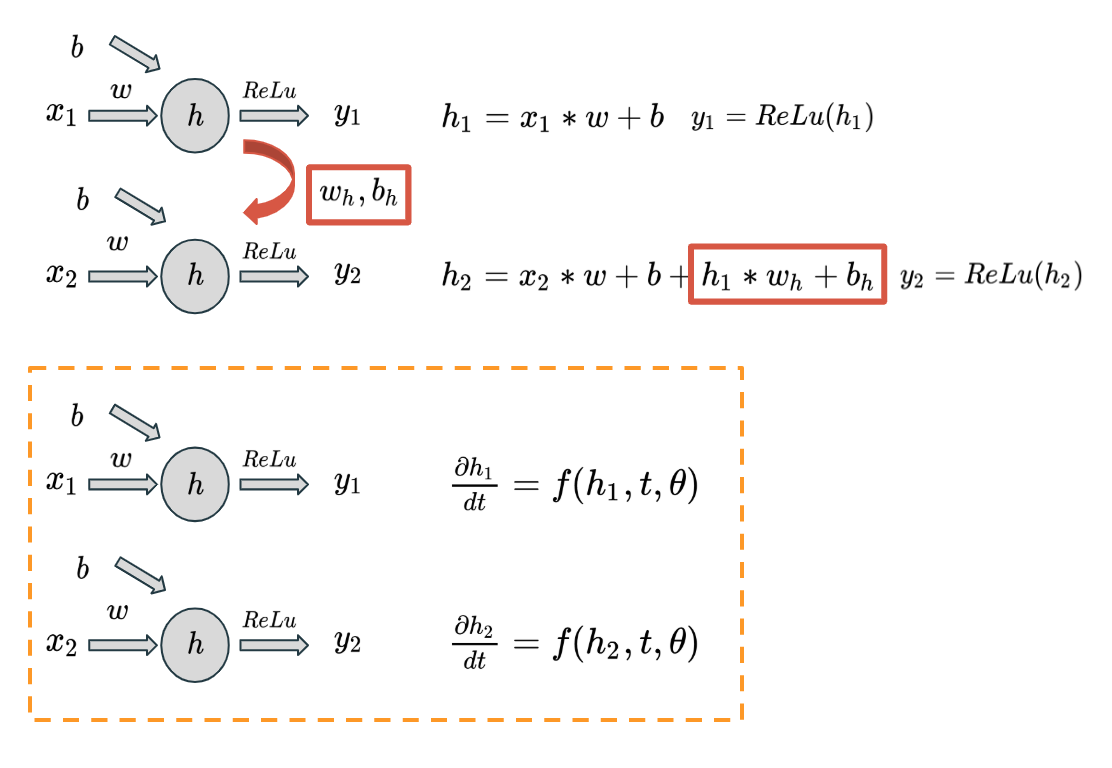
\includegraphics[width=.5\textwidth]{intro.png}}
\caption{Idea of RNN and NODE. $ReLu$ is activation function in neural network and $x_1, x_2...$ are input batch training data. The above figure is general RNN and the below(with orange rectangle) is NODE.}
\label{fig:rnn}
\end{center}
\vskip -0.05in
\end{figure}

Inspired by the fact that RNN need lots of memory storage, which is because we need to restore value of layer from last phase(especially, in some case, many phases in the past), novel ways to achieve RNN is introduced by Chen, called Neural Ordinary Differential Equations(NODE)\cite{Chen2018NeuralEquations}.

In this cases, the connection along temporal sequence is built by a differential equation, instead of a linear function shown as above equation (\ref{equ:rnn}):
\begin{equation}
    \label{equ:node}
    \frac{\partial h_t}{\partial t} = f(h_t, t, \theta)
\end{equation}
where $\theta$ and $f$ are given user-determined parameters and function. Starting from first phase $h_0$, we can define the value of layer in phase $t$, $h_t$, to be the solution of the equation. Figure (\ref{fig:rnn}) contrasts two approaches of both general RNN and NODE.

Defining and evaluating a model using NODE method have several benefits:
\begin{itemize}
    \item \textbf{Memory efficiency} In the third section, we will show that we don't need back-propagating through the operations of the solvers. That means it's unnecessary to store any intermediate data from forward pass. 
    
    \item \textbf{Adaptive computation} Euler's method would be one of the simplest method to solve Differential Equations. And many other methods for solving the problem are introduced recently\cite{Runge1895UeberDifferentialgleichungen, Shampine1987SolvingProblems}. That means we have many flexible choices to solve our NODE in neutral network.
    
    \item \textbf{Parameter efficiency} When the hidden unit dynamics are parameterized as a function in equation \ref{equ:node}, layers from different phases are tied together. Thus, parameters are reduced in neutral network.
    
    \item \textbf{Continuous time-series models} In usual recurrent neutral, the input data are discrete observation while the proposed method can incorporate data obtained from at arbitrary times.
\end{itemize}

This report basically introduces this novel recurrent neutral network method. In section (\ref{sec:related-work}), related works about different solver and learning strategy of differential equations will be introduced. The section (\ref{sec:methods}) will discuss NODE solvers. Experiment summary for Unsupervised Learning, Continuous Normalizing Flows and Generative Latent Function are shown in section (\ref{sec:experiment}). Finally, evaluation of experiements and limitations of NODE will be discussed in section (\ref{sec:discussion}).

\section{Related Works (by Zayid)}
\label{sec:related-work}
The characteristic features of this paper relied on past work to built upon in the areas of adjusting computation time, use of reversibility to reduce storage, learning differential equations, and differentiating ODE solvers. 
\subsection{Adaptive Computation}
Adaptive computation time was an algorithm that was discovered for the purposes of flexibly determining the amount of computational steps needed for going from input to output \cite{graves2016adaptive,jernite2016variable,figurnov2017spatially,chang2018reversible}. This method served as a means of improving performance of recurrent neural networks that would compute at a constant rate no matter the input.
\subsection{Reversible Architecture}
The modification of ResNets to have reversible architecture was a push to  avoid the bottleneck of memory capacity that occurs when networks get deeper and wider \cite{gomez2017reversible,ruthotto2018deep,chang2017multi}. The reversible architecture allowed for more efficient design by being able to compute activations in a current layer from the next layer hence limiting the amount of storage need. This did in fact increase some parameters that were not reversible. Ultimately, the authors of this paper were definitely inspired by this, however, they decided to lift restrictions placed on the architecture of prior reversible ResNets that resulted in partitioned hidden units.
\subsection{Learning Differential Equations }
As a major proponent of learning differential equations from data, Raissi (\citeyear{raissi2018multistep}) has connected components of machine learning to creating high complexity models. Others like Raissi
\cite{long2017pde} have used neural networks  with insufficient amount of data simply to build data-driven models outright. Furthermore, more research has been building to adding  Gaussian Processes to fit differential equations \cite{raissi2018multistep}.
\subsection{Differentiation through ODE Solvers}
The adjoint method for differentiation through ODE solvers in not original to the authors of this paper. Existing libraries such as the dolfin library \cite{farrell2013automated} and Stan library \cite{carpenter2015stan} implement some version of the adjoint method for solving ODEs and PDEs. Still, the authors decided to expand upon these methods by using a generic vector-Jacobian product for the use of general integration of black-box ODE solvers. 


\section{Methods (by Weijie)}
\label{sec:methods}
When training neutral network, we need to compute gradient for each layer by backpropagation, which means gradient passes from the last layer to the first layer. 
The main difficulty in the ODE method is how to perform backpropagation through ODE layers and solver. 

NODE approaches this by treating the solver as a black box (i.e. we do not need figure out how to actually solve the equation ($\ref{equ:node}$). 
Then, we compute compute gradients using the adjoint sensitivity method\cite{Chambers2006TheProcesses}. 

In adjoint sensitivity method, we need to formulate scalar-valued loss function $L()$ needed to be optimized as: 
$$
    L(z(t_1)) = L\bigg(z(t_0)+\int_{t_0}^{t_1}f(z(t), t, \theta)d t\bigg)
$$

To optimize $L$ by gradient method(like gradient descent), we need to compute gradient with respect to $\theta$. In first step, we should determine how value in state $t$, $z(t)$ affects value of loss function. It's called adjoint: $a(t)=\frac{\partial L}{\partial z(t)}$.

The paper\cite{Chen2018NeuralEquations} proves in the Appendix that (1) its dynamics are computed by another ODE. This ODE can be thought of as the instantaneous analog of the chain rule: 
$$
    \frac{\partial a(t)}{\partial t} = -a(t)^T\frac{\partial f(z(t), t, \theta)}{\partial z}
$$
and (2) the gradient of loss function is the integral of $\frac{\partial a(t)}{\partial t}$:
\begin{equation}
    \label{equ:method}
    \frac{\partial L}{\partial \theta} = - \int_{t_1}^{t_0}a(t)^T\frac{\partial f(z(t),t,\theta)}{\partial \theta}d t
\end{equation}
where the integral is computed starting from its final value $z(t_1)$ to initial value $z(t_0)$.

Basically, we can consider the adjoint as a ``state" or ``value" in each ODE layers. We accumulate information from all layers using integral operation, to estimate gradient of parameters. The figure (\ref{fig:method}) shows the whole idea discussed in this part.

\begin{figure}[ht]
\vskip 0.05in
\begin{center}
\centerline{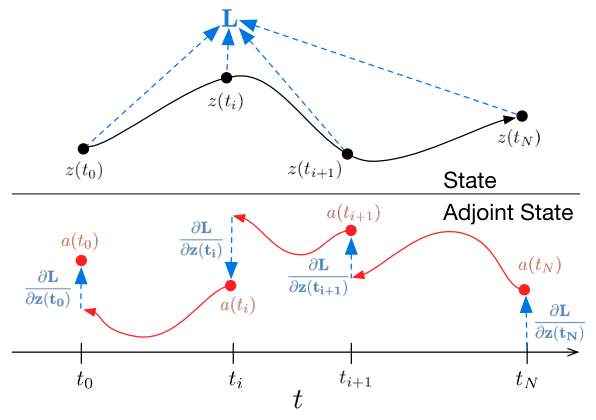
\includegraphics[width=.5\textwidth]{method.png}}
\caption{The UP figure shows each state in NODE affect the value of loss function and the DOWN figure indicates that how we can solve gradient of loss function by equation (\ref{equ:method}).}
\label{fig:method}
\end{center}
\vskip -0.05in
\end{figure}

\section{Experiments(by Zayid and Weijie)}
\label{sec:experiment}
NODE was used on three tasks to compare to other residual neural networks:
1) Supervised Learning , 2) Normalizing Flows, and 3) Generative Latent Function Time Series Model.
\subsection{Supervised Learning}
Supervised learning was done on the MNIST dataset using several other neural network architectures:  1-Layer MLP, ResNet, RK-Net, and ODE-Net. Performance between the models were compared on the measures of test error, number of parameters used, memory storage, and computation time. The ability to control error via tuning the tolerance of the true solution was also assessed.

\subsection{Normalizing Flows}
A normalizing flow is transformation of initial density into a more complex one by applying a sequence of invertible transformations until a desired level of complexity is attained. Discrete (NF) and continuous normalizing flows (CNF) were computed an compared for their ability to transform noise to data. The number of hidden units, M, for the CNF were varied and compared to an equivalent number of hidden layers, K, used for the NF.

\subsection{Generative Latent Function Time Series Model}
It's difficult to apply neutral network to irregularly-sampled data, such as medical records, network traffic or neural spiking data. In these cases, we can obtain only certain part of data along time series.

Our approach can be also used to address missing data using a generative time-series model. We can formulate each observed data in phase $t$ as state $x_t$. All $z_t$ connected with a differential equations with is similar with NODE, are time-continues data we need to solve. On the other word, we only obtain some data $x_t$ from $z$.

The observed data is related with state $h$ by likelihoods: $x_{t_i} = p(x | z_t, \theta)$.

\section{Discussion(by Zayid)}
\label{sec:discussion}
Overall, the authors evaluated the use of Black-Box ODE solvers for time-series modeling, supervised learning, and density estimation with flexible and fast computation. Also, a scaleable version of continuous-time normalizing flows was developed.

It is known that the key benefits of using ODE solvers is memory efficiency, adaptive computation, and parameter efficiency. One of the ways of achieving such a feat stems from the adjoint sensitivity method that computes gradients by solving a second, augmented ODE backwards in time, and is applicable to all ODE solvers. This approach scales linearly with problem size, has low memory cost, and explicitly controls numerical error.

In the supervised learning setting, ODE-Nets and RK-Nets achieved similar performance as the ResNet, while using fewer parameters which is critical in demonstrating how useful ODE-Nets can potentially be. Then, when experimenting with normalizing flows the authors observed that despite increasing the depth,K (layers) of the NF  and the width, M (hidden units) of the CNF result in better normalizing flows. This is notable because increasing the width of of a neural network is easier than increasing the depth.
Additionally, CNFs are reversible, so training can be done on a density estimation task and still be able to sample from the learned density efficiently. Lastly, in these classification and density estimation experiments, we were able to reduce the tolerance to 1e-3 and 1e-5, respectively, without degrading performance.

Finally, exploring time-series models, the authors found potential in NODE for applying neural networks to irregularly-sampled data such as medical records, network traffic, or neural spiking data that is rather difficult. Difficulties arise due missing data and ill-defined latent variables. However, missing data can be addressed using generative time-series models with NODE.

Granted NODE reveals exciting features, there were some limitations the authors disclosed. Mini-batching was shown to be a less straightforward approach here than for standard neural networks. In some cases, controlling error on all batch elements together required evaluating the combined system K times more often than if each system was solved individually.  When using ODEs it is also important to verify that a unique solution does in fact exist. The authors claim to verify this via Picard's Existence Theorem \cite{coddington1955theory}  only if the differential equation is uniformly Lipschitz continuous in z and continuous in t. This theorem holds for the authors' proposed model only if the neural network has finite weights and uses Lipshitz nonlinearities, such as tanh or relu.
Moreover, the potential for introducing numerical error into the backward propagation. The authors recommended in the future that if the reconstructed trajectory diverges from the original, then \textbf{checkpointing}, the act of storing intermediate values of z on the forward pass, and reconstructing the exact forward trajectory by re-integrating from those points, can alleviate these problems.


% In the unusual situation where you want a paper to appear in the
% references without citing it in the main text, use \nocite
\nocite{langley00}

\bibliography{refer}
\bibliographystyle{icml2019}

\end{document}
